\documentclass[10pt,a4paper]{article}
\usepackage[utf8]{inputenc}
\usepackage[english]{babel}
\usepackage{amsmath}
\usepackage{amsfonts}
\usepackage{amssymb}
\usepackage{graphicx}
\usepackage{indentfirst}
\usepackage{fancyvrb}
\usepackage{subfigure}
\usepackage{enumitem}
\usepackage{booktabs}
\usepackage[hidelinks]{hyperref}
\author{Giuseppe L'Erario}
\date{}
\title{Bayesian Networks}

\begin{document}
	\maketitle
	
\section*{Introduction}
A \emph{Bayesian network} is a graphical model used for the analysis of probabilistic relationship between events, represented by variables.

Every variable is sketched by a node and the nodes are connected by arrows, representing the relationship between the variables.

In this report, in particular, there will be analysed three problems with the help of \emph{Belief and decision network Tool}:
\begin{itemize}
	\item weather problem;
	\item coins problem;
	\item fire alarm problem.
\end{itemize}

\section{Weather problem}

The Bayesian network corresponding to the problem is shown in fig.\ref{weather_prob}.

\begin{figure}[h]
	\centering
	\subfigure[Network.\label{netw_weath}]{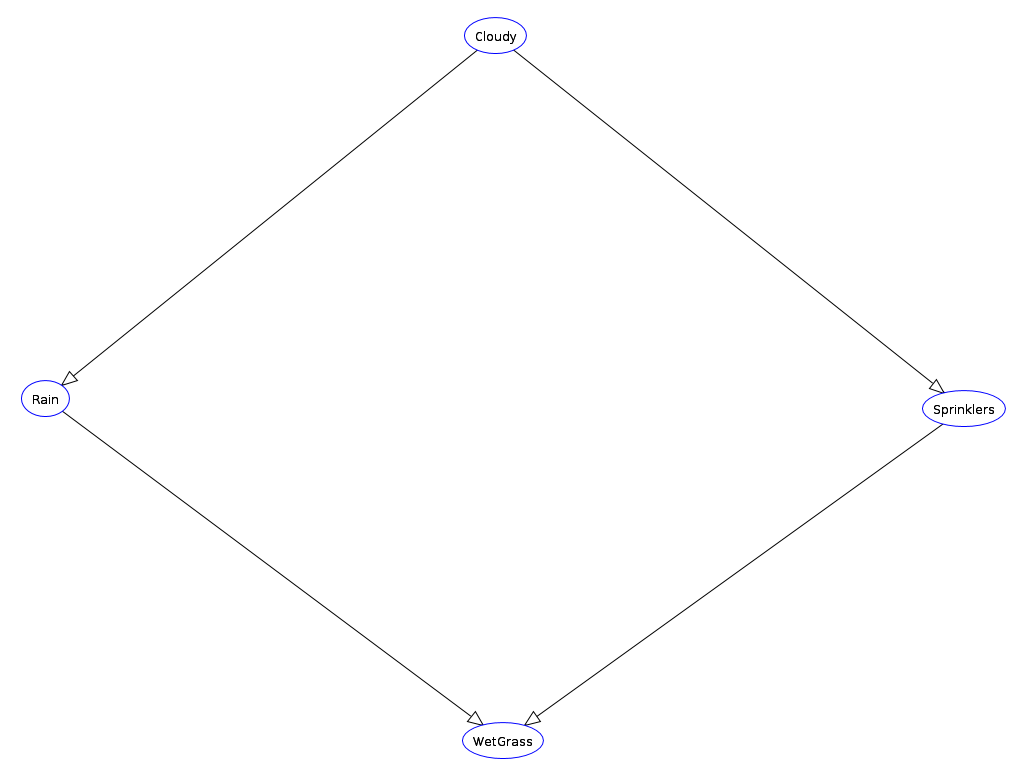
\includegraphics[width=0.4\linewidth]{../Rain}}\qquad
	\subfigure[Probability.\label{prob_weath}]{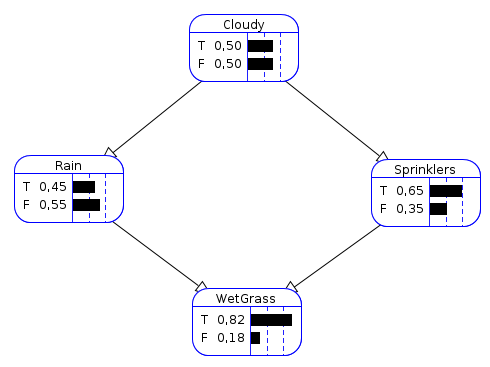
\includegraphics[width=0.4\linewidth]{../Rain_joint}}
	\caption{Bayesian network relative to weather problem.\label{weather_prob}}
\end{figure}

In fig.\ref{prob_weath} there are the probabilities of every event in absence of observations.

By the chain rule and exploiting the conditional independence we can obtain the joint probability:
\begin{align*}
P(W,R,S,C)=P(W|R,S,C) P(R|S,C)P(S|C)P(C)  \\ 
\Rightarrow P(W,R,S,C)=P(W|R,S)P(R|C)P(S|C)P(C)
\end{align*}

We introduce two observations: \emph{WetGrass=True} and \emph{Cloudy=False}. As it can be seen in fig.\ref{fig:Rain_solved}, the probability it rained is $P(R)=0.12$ and the probability the sprinklers were on is $P(S)=0.99$

\begin{figure}
\centering
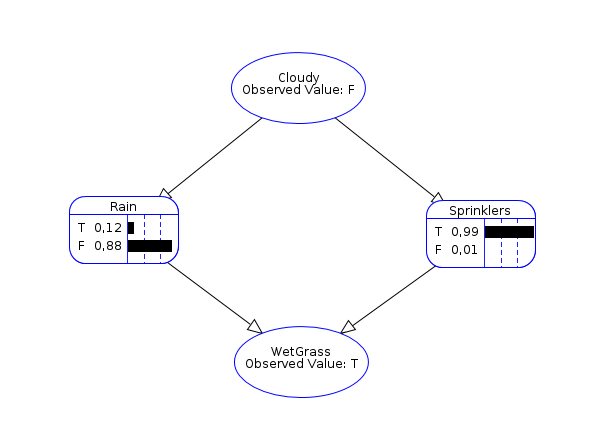
\includegraphics[width=0.7\linewidth]{../Rain_solved}
\caption{Probability with observations.}
\label{fig:Rain_solved}
\end{figure}

\section{Coin problem}

There are three biased coins. Every coin has equal probability to come out (1/3 each) but different probability to come up head:
\begin{itemize}
	\item Coin 1: 20\%
	\item Coin 2: 60\%
	\item Coin 3: 80\%
\end{itemize}  	

\begin{figure}[h]
\centering
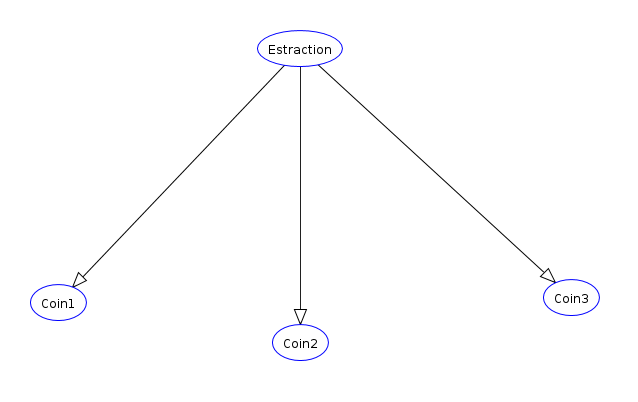
\includegraphics[width=0.7\linewidth]{../Coin}
\caption{Bayesian network of coins problem.}
\label{fig:Coin}
\end{figure}

We can set the associated probability with the tool, as in fig.\ref{fig:Coin_prob}.

\begin{figure}
\centering
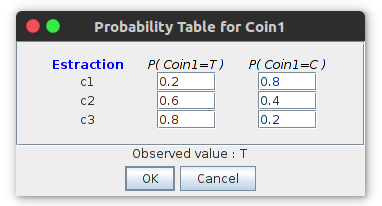
\includegraphics[width=0.7\linewidth]{../Coin_prob}
\caption{Probability of extraction.}
\label{fig:Coin_prob}
\end{figure}

After the observations (head twice and tails once) comes out that the coin that, most likely, gives this result is the second (fig.\ref{fig:Coin_solved}).

\begin{figure}
\centering
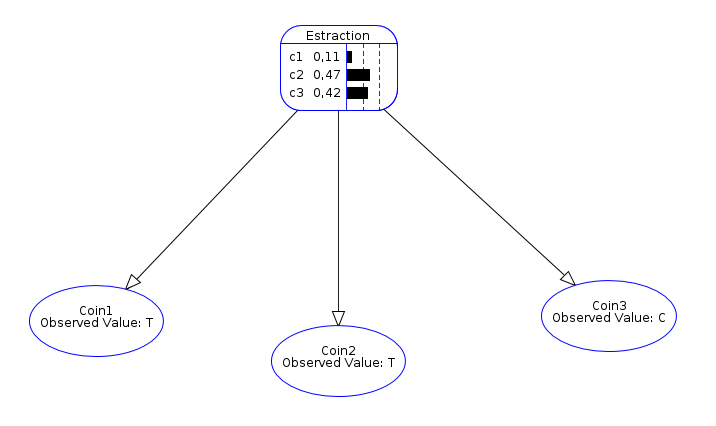
\includegraphics[width=0.7\linewidth]{../Coin_solved}
\caption{The solved Bayesian network.}
\label{fig:Coin_solved}
\end{figure}

\section{Fire alarm problem}

The joint probability of the \emph{fire alarm problem} is calculated as in the \emph{weather problem}:
\begin{align*}
P(R,L,A,S,T,F) = P(R|L)P(L|A)P(A|T,F)P(S|F)P(T)P(F)
\end{align*}

The associated graph, with the extension \emph{CallMom} if the alarm goes off is in fig.\ref{fig:Fire_alarm}.
\begin{figure}
\centering
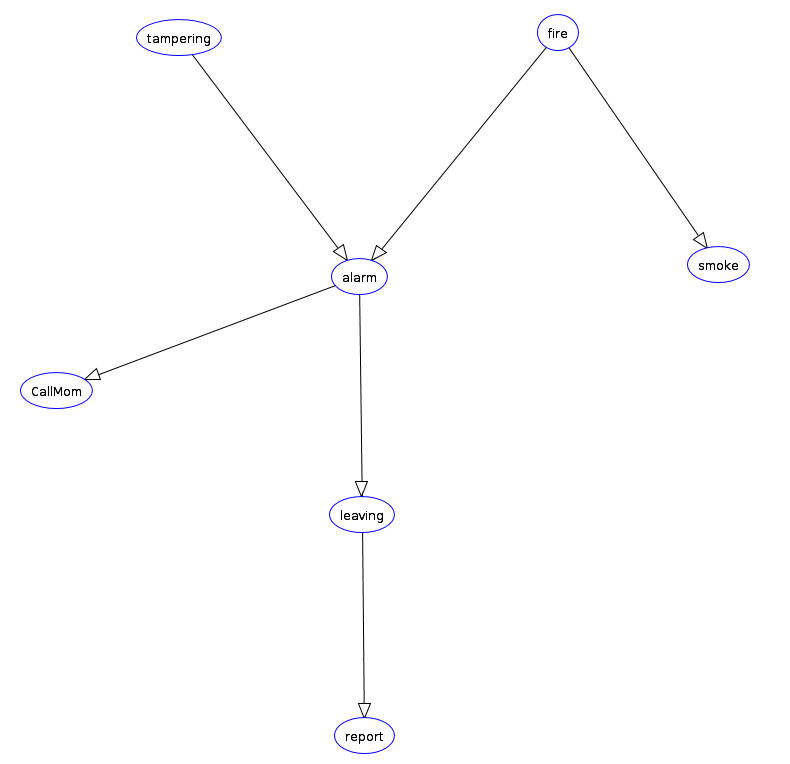
\includegraphics[width=0.7\linewidth]{../Fire_alarm}
\caption{}
\label{fig:Fire_alarm}
\end{figure}


\end{document}